%
% File acl2018.tex
%
%% Based on the style files for ACL-2017, with some changes, which were, in turn,
%% Based on the style files for ACL-2015, with some improvements
%%  taken from the NAACL-2016 style
%% Based on the style files for ACL-2014, which were, in turn,
%% based on ACL-2013, ACL-2012, ACL-2011, ACL-2010, ACL-IJCNLP-2009,
%% EACL-2009, IJCNLP-2008...
%% Based on the style files for EACL 2006 by 
%%e.agirre@ehu.es or Sergi.Balari@uab.es
%% and that of ACL 08 by Joakim Nivre and Noah Smith

\documentclass[11pt,a4paper]{article}
\usepackage[hyperref]{acl2018}
\usepackage{times}
\usepackage{latexsym}
\usepackage{amsmath}
\usepackage{url}

\usepackage{tabularx}

\usepackage{graphicx}
\graphicspath{ {graphics/} }

\aclfinalcopy % Uncomment this line for the final submission
%\def\aclpaperid{***} %  Enter the acl Paper ID here

%\setlength\titlebox{5cm}
% You can expand the titlebox if you need extra space
% to show all the authors. Please do not make the titlebox
% smaller than 5cm (the original size); we will check this
% in the camera-ready version and ask you to change it back.

\newcommand\BibTeX{B{\sc ib}\TeX}

\title{Movise Domain Bot \\ Final project}

\author{Andrea Tupini \\
  MAT.  194578 \\
  {\tt andrea.tupini@studenti.unitn.it}}

\date{}

\begin{document}
	
\maketitle

\begin{abstract}
	
	abstract. 
	\\
	
\end{abstract} 

\section{Introduction}

Introduction

	
\section{Data Analysis}
\label{sec-data-analysis}

	data:
	
	\begin{description}
		\item[NLSPARQL.test] words and IOB tags for testing
		\item[NLSPARQL.train] words and IOB tags for training              
		\item[NLSPARQL.test.feats] words, POS tags and lemmas for testing
		\item[NLSPARQL.train.feats] words, POS tags and lemmas for training
	\end{description}

	
	\hspace*{-0.4cm}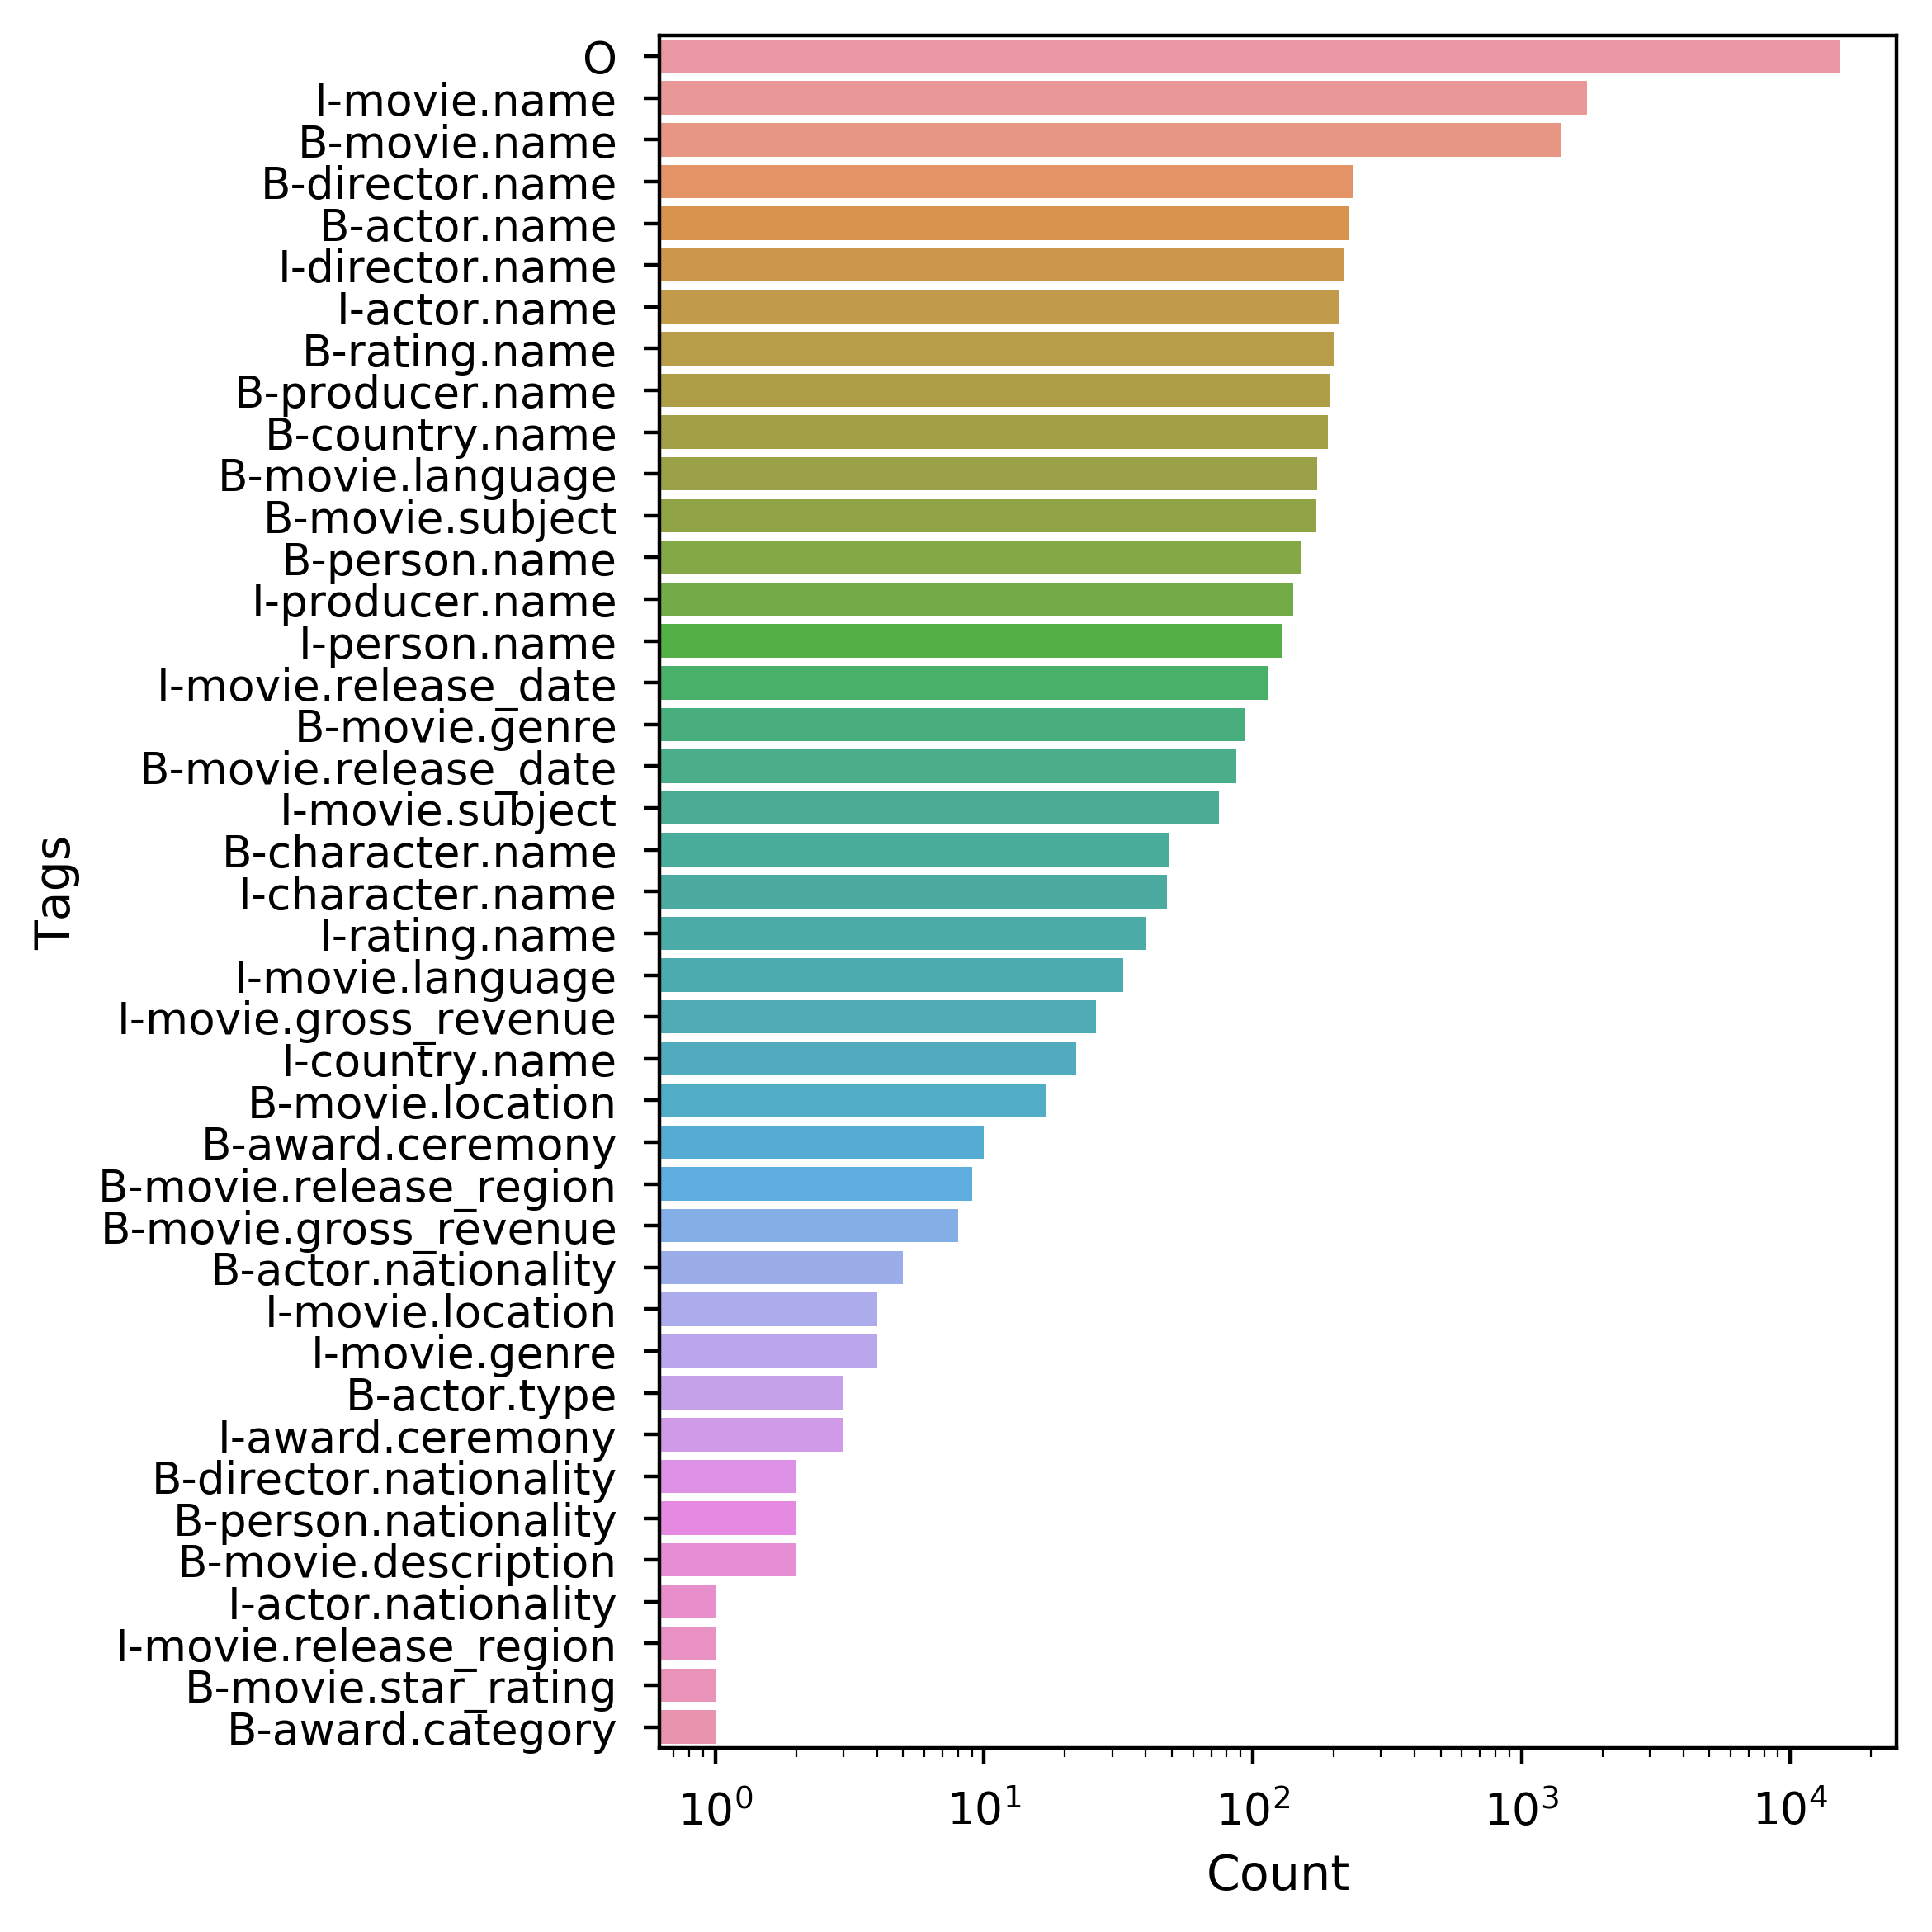
\includegraphics[scale=0.5]{barplot_iob_tag_counts}



\section{Evaluation}
	
	ev

\subsection{NLU Module}

	lu module
	

\section{Future Work}

	fw.
	

\section{Conclusion}
	
	


% include your own bib file like this:
\bibliographystyle{plain}
%\bibliography{acl2018}

%\bibliographystyle{plainnat}
\bibliography{bibliography}

%\bibliographystyle{acl_natbib}


\end{document}
